\documentclass[a4paper]{ctexrep}

\usepackage{tikz}
\usepackage[version=4]{mhchem}
\usepackage{graphicx}
\usepackage{float}
\usepackage{xcolor}
\usepackage{mathtools}
\usepackage{booktabs}

\newcommand{\mol}{\mathrm{mol}}
\renewcommand{\d}{\mathrm{d}}

\newtheorem{definition}{定义}[chapter]
\newtheorem{example}{例}[chapter]
\newenvironment{solution}{\par \noindent \textbf{解}  \par \vspace{0.3em}}{\par}
\newtheorem{question}{习题}[chapter]

\graphicspath{ {./img} }

\author{Y.C. Long}
\title{物理化学 -- 刘婧媛}

\begin{document}
    % 作业 20%
    % 课程报告 10%
    % 期末考试 70%
    \maketitle
    \tableofcontents

    \chapter{电解质溶液}
        \section{前言}
        \subsection{电化学综述}
        内容:$\mbox{化学反应} \leftrightarrow \mbox{电现象}$。既包括热力学问题,也包括动力学问题。电化学的用途主要包括研究化学能和电能的互相转换:
        \[
            \mbox{化学能} \ce{<=>T[\mbox{电池}][\mbox{电解池}]} \mbox{电能}  
        \]

        电化学系统就是电池或电解池,由导体或半导体组成,多相存在,为科学研究以及生产过程提供精确快速地研究测定方法。
        \subsection{电解质溶液}的
        电解质溶液是电池和电解池的重要组成部分。
        \subsubsection{与非电解质溶液的区别}
        \paragraph{导电} 物理动力学 

        \paragraph{热力学} 高度不理想性
        \subsubsection{电解质溶液的特点}
        电解质溶液的概念较多,要以理解为主。

        \section{电化学中的基本概念}

        \subsection{电解质溶液的导电机理(The mechanism of conduction for electrolyte solution)}
        金属(第一类导体)和电解质溶液(第二类导体)的导电机理不同。例如,电解$\ce{CuCl2}$溶液(如图\ref{fig:transfer}),首先有离子电迁移的物理变化,后有电极反应的化学变化。

        \begin{figure}[h]
            \centering
            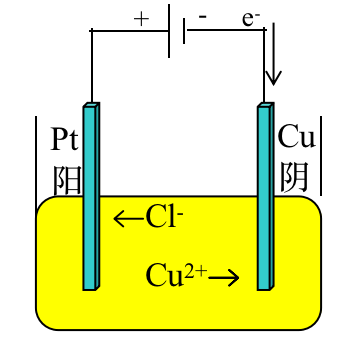
\includegraphics[width=0.3\textwidth]{transfer.png}
            \caption{$\ce{CuCl2}$溶液通电后的情况}
            \label{fig:transfer}
        \end{figure}

        $\ce{Pt}$电极:$\ce{2Cl- -> Cl2 + 2e-}$ (氧化)

        $\ce{Cu}$电极:$\ce{Cu2+ + 2e- -> Cu}$(还原)

        总结果: $\ce{\mbox{电池(-)} ->T[e-] Cu ->T[e-][re] sln ->T[e-][ox] Pt ->T[e-] \mbox{电池(+)}}$

        \subsubsection{电极命名法}
        \paragraph{按电位高低} 电位高 -- 征集, 电位低 -- 负极

        \paragraph{按反应性质} 氧化 -- 阳极,还原 -- 阴极

        \section{Faraday电解定律}
        Faraday 归纳了多次实验结果,于1833年总结出了电解定律:
        \begin{enumerate}
            \item 电解界面上发生的化学变化物质的量与通入的电荷量成正比
            \item 若将几个电解池相连,通入等量的电荷,他们发生化学反应的物质的量相等
        \end{enumerate}

        \subsection{Faraday 常数}
        人们把在数值上等于1 mol元电荷的电量称为Faraday常数。Faraday常数需要记忆:$F \approx 96500 \mathrm{C} \cdot \mbox{mol}^{-1}$

        如果在电解池发生如下反应:
        \[ 
            \ce{M^{z+} + z_{+}e- -> M(s)}
        \]
        电子得失的化学计量数为$z_{+}e-$,则需要的电荷量为:$\ce{z_{+}e-} \cdot \mathrm{F}$

        \subsection{荷电粒子基本单位的选取}

        $n = \frac{N}{L}$,其中$N$为基本单元的个数,所以$n$值与基本单元有关,例如18g水,可以表示为:
        $n \ce{H2O} = 1 \mol$,$n(\ce{2H2O}) = 0.5 \mol$。
        在研究电解质溶液导电性质时,习惯用一个元电荷($\ce{e-}$)为基础指定物质量的基本单元。

        \paragraph{基本阴阳离子的基本单位}

        离子$\ce{M^{z+}}$ 用$n \left( \frac{1}{z_{+}} M^{z+}\right)$描述离子的物质的量。
        
        例 $n(\ce{H+})$,$n(\frac{1}{2}\ce{Cu^{2+}})$,$n(\frac{1}{3}Fe^{3+})$。

        这样做的好处是,$1 \mol$任何离子所带的电量均为$6.023 \times 10^{23} e$。

        \paragraph{电解质的基本单位}
        电解质$M_{\nu_+}A_{\nu_-}$,电离方程式为
        \[
            M_{\nu_+}A_{\nu_-} \ce{->T[电离]} \nu_+M^{z+} + \nu_-M^{z-}
        \]
        用$n \left( \frac{1}{z_+ \nu_+} M_{\nu_+}A_{\nu_-} \right)$。这样做的好处是

        \begin{enumerate}
            \item $1 \mol$任何物质全电离均产生$6.023 \times 10^{23} e$的正电荷和负电荷。
            \item 同一溶液中,电解质全电离时,有
            \[
                n \left( \frac{1}{z_+ \nu_+} M_{\nu_+}A_{\nu_-} \right) = n \left( \frac{1}{z_+} M^{2+} \right) = n  \left( \frac{1}{|z_-|} M^{2+} \right)
            \]
        \end{enumerate}

        \paragraph{参与氧化还原反应的物质M}

        $\ce{M + ze- ->T[re] M^{z-}}$,以$n \left( \frac{1}{z}M\right)$ 来描述物质M的物质的量

        \subsection{电流效率}

        电流效率为按照Faraday电解定律计算出来的理论电荷量于实际电荷量之比。

        \[
            \mbox{电流效率} = \frac{\mbox{Faraday定律计算的理论电荷量}}{\mbox{实际流过的电荷量}}  
        \]

        \section{离子的电迁移率和迁移数}

        \subsection{离子的电迁移率}
        
        \[
            \mbox{电解质} \ce{ ->T[电离] } \mbox{离子B} + \mbox{离子D}  
        \]

        \subsubsection{定义}

        通常讨论在一定$T$,$p$下的某一指定溶液,则离子迁移速率\[r_B = u_B\frac{\d E}{\d l}\],这里的$u_B$就是离子的电迁移率。也就是单位电位梯度下时,离子的迁移速度。

        \subsubsection{淌度的测量}

        根据定义,设法测定$r_{B}$和$E$

        \subsubsection{离子的极限电迁移率}
        
        在无限稀薄溶液中,离子的电迁移率称为极限电迁移率$u_B^{\infty}$,反应离子的基本特征,是离子的固有属性。

        \subsection{离子迁移数}

        电解质溶液导电时离子的具体迁移情况(Hittorf模型,见图\ref{fig:u_B}),把电解池分为阳极区,中间区,阴极区。离子B的迁移数是离子B运载的电荷量和总电流之比。

        \[
            t_B \overset{\mathrm{def}}{=} \frac{I_B}{I}
        \]
        
        \subsubsection{电迁移的相关结论}

        \begin{figure}[h]
            \centering
            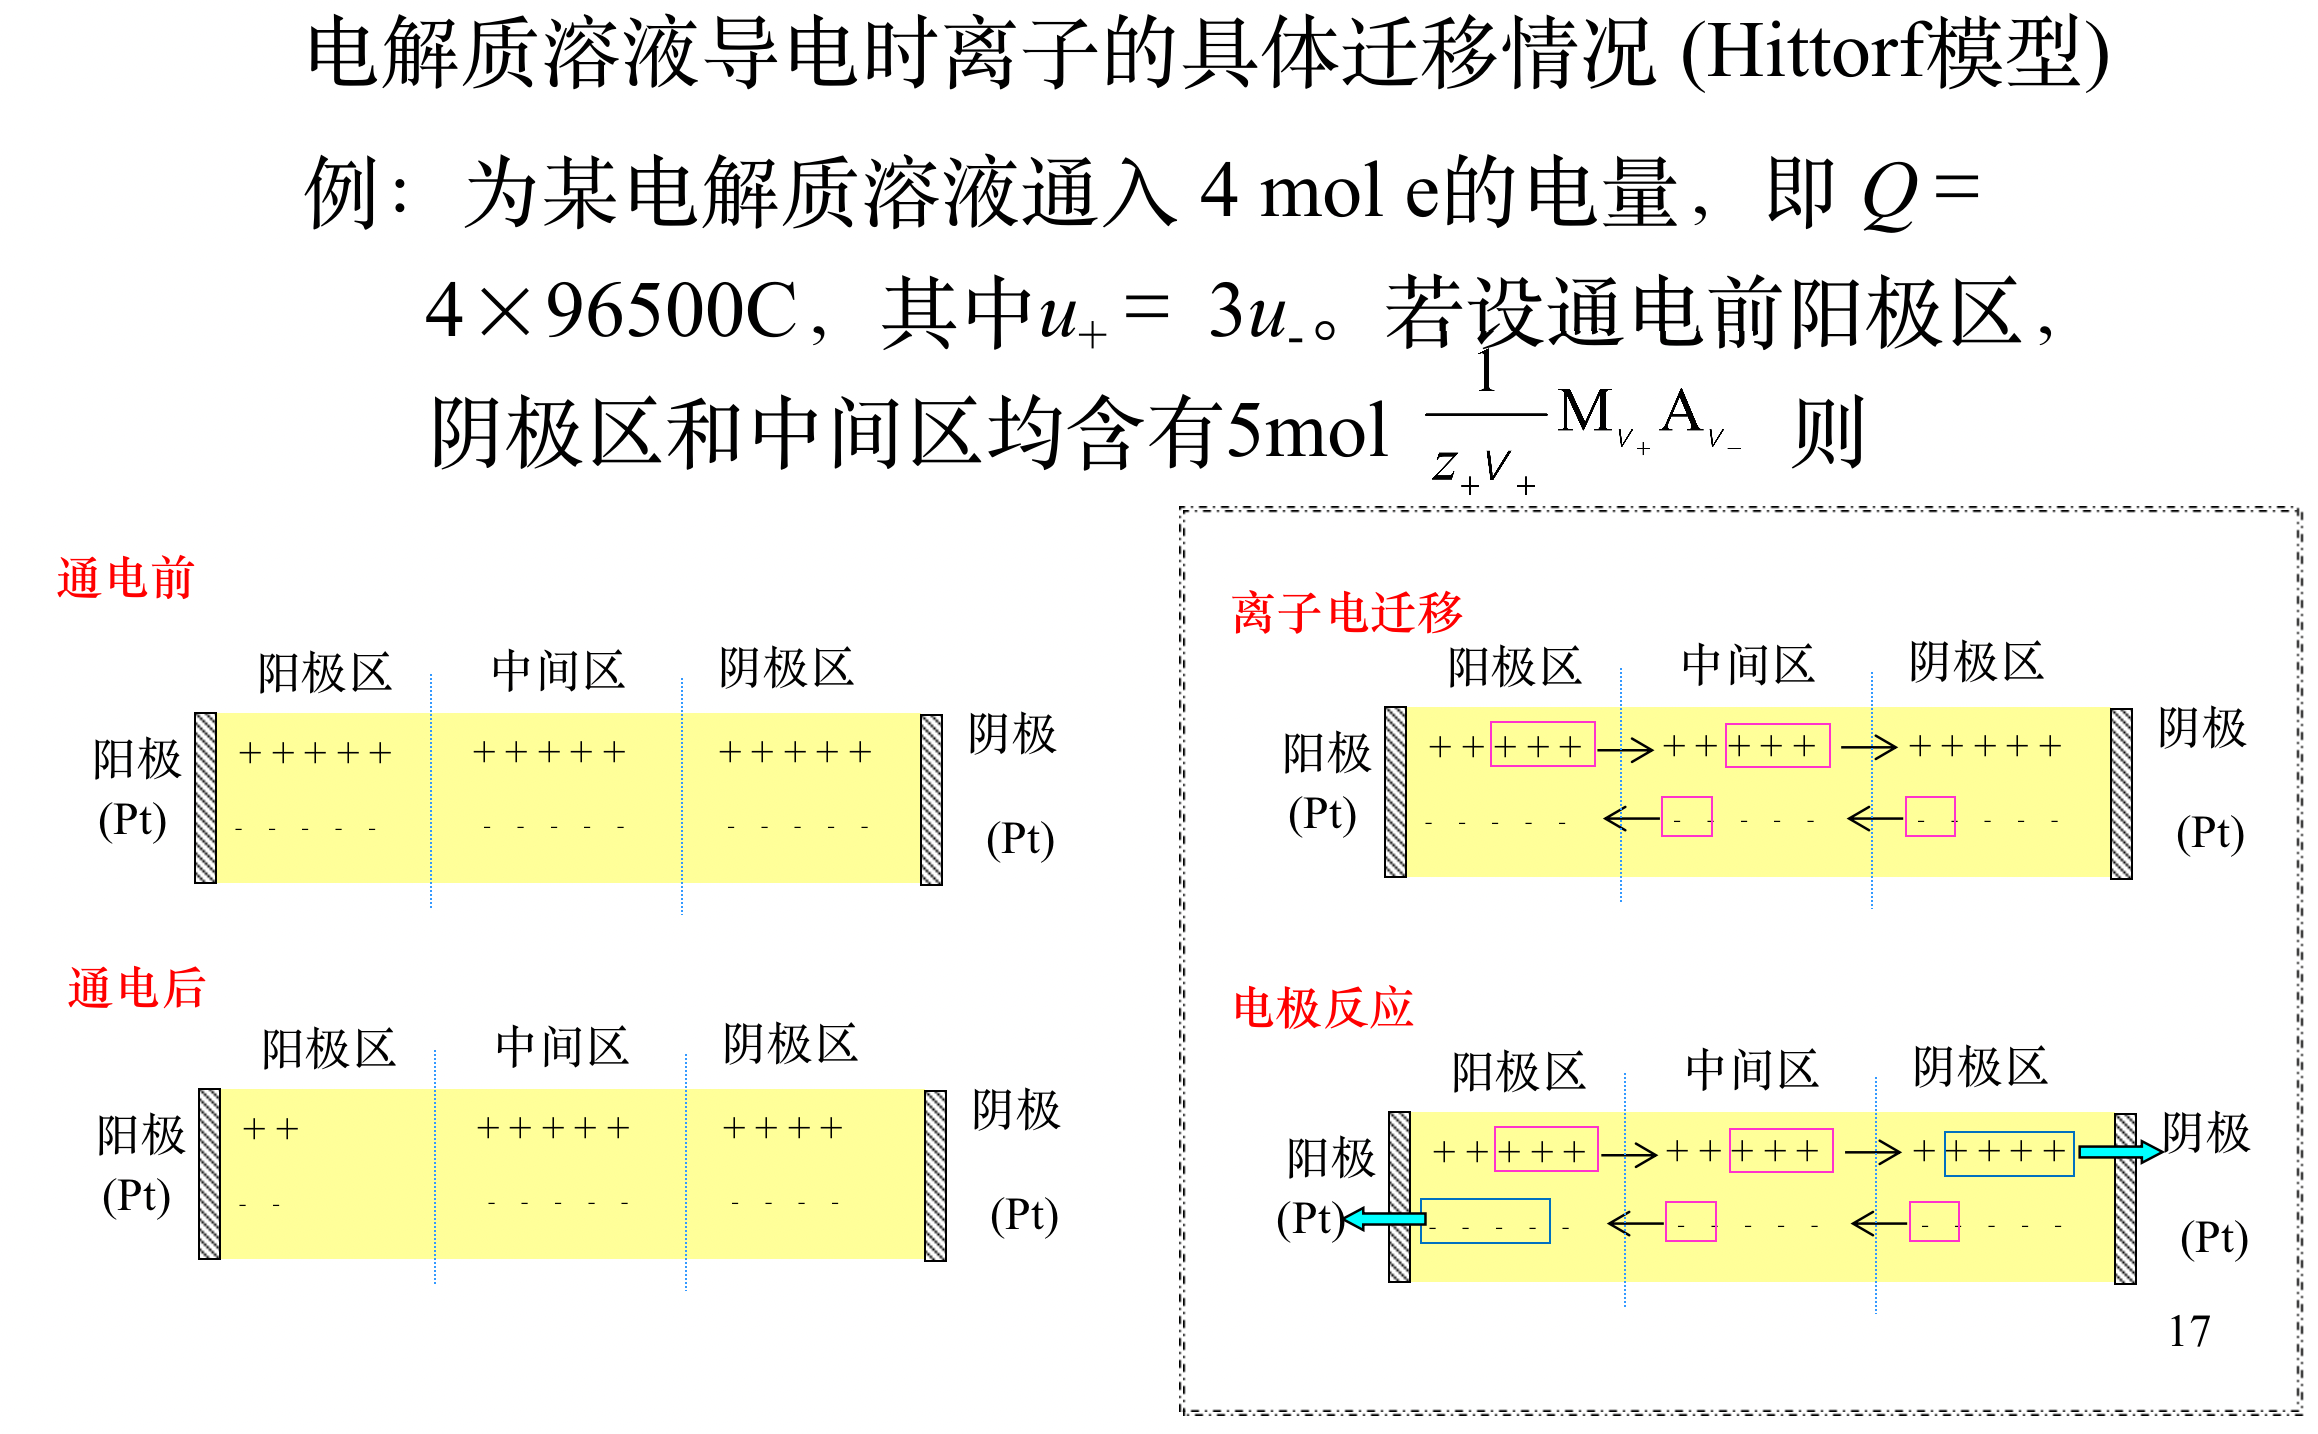
\includegraphics[width=1.0\textwidth]{u_B.png}
            \caption{运动情况}
            \label{fig:u_B}
        \end{figure}

        \paragraph{浓度变化} 中间区的浓度不变,两极区的浓度改变。
        \paragraph{物质的量关系} $n_B(\mbox{迁移}) \neq n_B(\mbox{电极反应})$
        \paragraph{溶液的导电任务由正负离子共同分担}
        \[
            \frac{t_{+}}{t_{-}} = \frac{u_{+}}{u_{-}}  
        \]

        \subsection{迁移数的测定}

        原理:

        \[
            t_B = \frac{Q_B}{Q}  
        \]
        \section{电解质溶液的电导}

        \subsection{电导和电导率}

        对金属导体,习惯用$R$表示导电能力$R = \rho \frac{l}{A}$,对电解质溶液,习惯用$\frac{1}{R}$,即:
        
        \[
            G = \frac{1}{R} = \frac{1}{\rho}\frac{A}{l} G = \kappa \frac{A}{l}  
        \]

        $G$,电导,$\kappa$,电导率

        $\kappa$ 一般与浓度$c$有关,强电解质中$\kappa$通常是浓度的单峰函数。在弱电解质中,$\kappa$与$c$的关系很小。

        \subsection{摩尔电导率}

        \begin{definition}
            \[
                \varLambda_m = \frac{\kappa}{c} 
            \]
        \end{definition}

        \subsubsection{$\varLambda_m$的物理意义}

        \[
            \varLambda_m = \frac{\kappa}{c} = \frac{G}{n}l^2  
        \]

        1 $\mol$ 的电解质置于两个相距 1 $\mathrm{m}$ 的平行电解板之间,此时溶液所具有的电导。

        强电解质的在$c$通常与$\varLambda_m$负相关,浓度越低,摩尔电导率越高。在弱电解质中,$\varLambda_m \sim \sqrt{c}$近似双曲线。在稀溶液范围内,$\varLambda_m$对$c$十分敏感。弱电解质必须考虑离子数的影响,在稀溶液低浓度的情况下,弱电解质的电离度越来越大,离子数不断增加,导电性增强。总的而言,在强电解质中,主要考虑的是淌度$u_B$的影响,弱电解质中,还需要考虑电离度$\alpha$的影响。

        $\varLambda_m$不是电解质的本性。

        \subsubsection{极限摩尔电导率}

        Kohlrausch经验规则

        \[
            \varLambda_m = \varLambda_m^\infty (1 - \beta \sqrt{c})
        \]

        其中

        \[
            \varLambda_m^\infty = \lim_{c \rightarrow 0} \varLambda_m   
        \]

        $\varLambda_m^\infty$代表离子间无静电作用时$1 \mol$电解质的(最大)导电能力,所以$\Lambda_m ^\infty$是电解质导电能力的标志。$\varLambda_m (298\mathrm{K})$ 可查手册。强电解质$\varLambda_m^\infty$ 可由实验外推。

        \subsubsection{摩尔电导率的测量}

        $\varLambda_m$与其他电学量一样,可以通过基本电学量$I$,$U$,$R$,$Q$等的测量求得。不通电的是应该在电导池中测量。

        原理:$\varLambda_m = \frac{\kappa}{c} $

        求$\kappa$,
        
        \[
            \kappa = G \frac{k}{A} = \frac{1}{R} \frac{l}{A} = \frac{K_{cell}}{R}  
        \]

        $K_{cell}$可以由某个$\kappa$已知的溶液$\ce{KCl}$ 测其电阻求得。现在多用电导率仪直接测量$\kappa$

        \subsubsection{基本质点的选取}

        摩尔电导率必须对应溶液中含有$1 \mol$电解质,但对电解质基本质点的选取取决于研究需要。在做题的时候必须说明选的基本质点是什么,比如$\varLambda_m (\ce{CuSO4})$ 或者 $\varLambda_m (\ce{2CuSO4})$

        \section{单个离子对电解质溶液的导电能力的贡献}

        \subsection{导电能力的加和性}

        \subsubsection{$G$的加和性}

        $Q = Q_+ + Q_-$ 正负离子相当于并联

        \subsubsection{$\kappa$的加和性}

        \[
            G = \kappa \frac{A}{l}  
        \]

        \[
            \kappa = c\alpha(u_+ + u_-)F  
        \]

        \[
            \kappa_+ = c_+ u_+ F  
        \]

        \[
            \kappa_- = c_- u_- F  
        \]

        \begin{equation*}
            A_{m,+} = u_+ F
        \end{equation*}

        \subsubsection{$\varLambda_m$的加和性}

        \begin{definition}
            \[
                \varLambda_{m, +} = \frac{\kappa_+}{c_+}  
            \]
        \end{definition}

        \[
            \varLambda_m = \frac{\kappa}{c} = \frac{\kappa_+ + \kappa_-}{c}  
        \]

        \[
            \varLambda_m = \alpha \varLambda_{m, +} + \alpha \varLambda_{m, -}
        \]

        \[
            \varLambda_{m, +} = t_+ \varLambda_{m}  
        \]

        \[
            \varLambda_{m, -} = t_- \varLambda_{m}  
        \]

        \subsubsection{离子的极限摩尔电导率}

        \[
            \varLambda_m^\infty = \varLambda_{m, +}^\infty + \varLambda_{m, -}^\infty
        \]

        \paragraph{独立迁移定律} 在无限稀释的溶液中,每种离子独立移动,不受其他离子影响,电解质的无线稀释摩尔电导率可以认为是独立的性质。

        弱电解质的$\varLambda_m^\infty$ 可以直接查表,可以通过测强电解质的$\varLambda_m^\infty$求得:

        \begin{align*}
            \varLambda_m^\infty{HAc} &= \varLambda_{m, +}^\infty(\ce{H+}) + \varLambda_m^\infty(\ce{Ac-}) \\
            &= \varLambda_m^\infty{\ce{HCl}} + \varLambda_m^\infty{\ce{NaAc}} - \varLambda_m^\infty{\ce{NaCl}}
        \end{align*}
    
    \section{电导法的应用}


    \subsection{检测水的纯度}

    \begin{table}[h]
        \centering
        \begin{tabular}{ll}
            \toprule
            \textbf{水} & \textbf{电导率} \\
            \midrule
            普通蒸馏水 & $ 1 \times 10^{-3} \mathrm{S \cdot m^{-1}} $ \\
            去离子水 & $ 1 \times 10^{-4} \mathrm{S \cdot m^{-1}} $ \\
            理论纯水 & $ 5.5 \times 10^{-6} \mathrm{S \cdot m^{-1}} $ \\
            \bottomrule
        \end{tabular}
    \end{table}

    \subsection{弱电解质电离常数的测定}
    对于一般的弱电解质,离子间静电引力晓得可以忽略$u_B \approx u_B^{\infty}$,所以

    \[
        \varLambda_m^{\infty} = (u_+^{\infty} + u_-^\infty)F 
    \]

    \[
        \alpha = \frac{\varLambda_m}{\varLambda_m^\infty}        
    \]


    \subsection{难溶盐的溶解度}

    难溶盐的强电解质:
    
    \[
        \varLambda_m = \varLambda_m^\infty  
    \]

    难溶盐本身的电导率很低,这个时候水的电导率就不可忽略。

    \[
        \kappa_{\mbox{难溶盐}} = \kappa_{\mbox{溶液}} - \kappa_{\ce{H2O}}  
    \]

    用摩尔电导率的公式即可求得难溶盐饱和溶液的浓度

    \[
        \varLambda_{m\mbox{难溶盐}} = \frac{\kappa_{\mbox{难溶盐}}}{c} = \frac{\kappa_{\mbox{溶液}} - \kappa_{\ce{H2O}}  }{c}
    \]

    \subsection{电导滴定}

    \section{电解质的平均活度和平均因子}

    \subsection{电解质的化学势}

    理想溶液某一组分$B$的化学势:

    \[
        \mu_B = \mu_B^\ominus(T) + RT\ln \frac{m_B}{m^\ominus} 
    \]

    非理想溶液某一组分的化学势:

    \[
        \mu_B = \mu_B^\ominus(T) + RT\ln a_{B,m} 
    \]

    其中
    
    \[
        a_{B,m} = \gamma_{B,m} \frac{m_b}{m^\ominus}    
    \]

    我们抽象地把阴离子和阳离子分开来看,也就是写出``阳离子化学势''和``阴离子化学势''。

    \[
        \mu_+ = \mu_+^\ominus(T) + RT\ln a_+ 
    \]

    \[
        \mu_- = \mu_-^\ominus(T) + RT\ln a_-  
    \]

    整体活度与实际存在的离子活度之间的关系:

    \[
        a_B = a_+^{\nu_+}a_-^{\nu_-}  
    \]

    \subsection{离子的平均活度和平均活度系数}

    \[
        a_B = a_+^{\nu_+}a_-^{\nu_-}  
    \]

    \[
        a_+ = \gamma_+ \frac{m_+}{m^\ominus}  \qquad a_- = \gamma_-  \frac{m_-}{m^\ominus}  
    \]

    $\gamma_+$和$\gamma_-$的数量无法测定,但是可以测定两者的平均值。这里的平均值是几何平均值。

    \[
        a_\pm \overset{\mathrm{def}}{=} (a_+^{\nu_+}a_-^{\nu_-})^\frac{1}{\nu} 
    \]

    \[
        \gamma_\pm \overset{\mathrm{def}}{=} (\gamma_+^{\nu_+}\gamma_-^{\nu_-})^\frac{1}{\nu}   
    \]

    \[
        m_\pm \overset{\mathrm{def}}{=} (m_+^{\nu_+}m_-^{\nu_-})^\frac{1}{\nu}   
    \]

    满足关系:

    \[
        a_\pm = \gamma_\pm \frac{m_\pm}{m^\ominus}
    \]

    $\gamma_\pm$可以直接由公式计算,也可以由实验测得。

    \chapter{可逆电池的电动势及其应用}

    \chapter{电解和极化作用}

    \chapter{化学反应动力学}

    \chapter{表面物理化学}

    \chapter{胶体化学}
\end{document}